\begin{figure}[htbp]
	\centering
	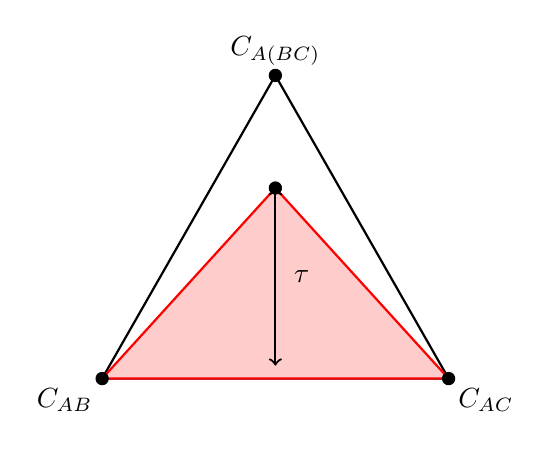
\begin{tikzpicture}[scale=1.1]
		\draw[thick] (0,0) -- (4,0) -- (2,3.5) -- cycle;

		\draw[thick, red, fill=red!20] (0,0) -- (4,0) -- (2,2.2) -- cycle;

		\node[below left] at (0,0) {$C_{AB}$};
		\node[below right] at (4,0) {$C_{AC}$};
		\node[above] at (2,3.5) {$C_{A(BC)}$};

		\draw[<->, thick] (2,0.15) -- (2,2.2) node[midway, right=3pt] {$\tau$};

		\draw[fill=black] (0,0) circle (2pt);
		\draw[fill=black] (4,0) circle (2pt);
		\draw[fill=black] (2,3.5) circle (2pt);
		\draw[fill=black] (2,2.2) circle (2pt);

	\end{tikzpicture}
	\caption{Coffman-Kundu-Wootters (CKW) inequality for three qubits. The squared entanglement $C_{A(BC)}^2$ (hypotenuse) must be at least as large as the sum $C_{AB}^2 + C_{AC}^2$ (base). The red region shows the tangle $\tau$, representing genuine tripartite entanglement not captured by pairwise measures.}
	\label{fig:ckw-inequality}
\end{figure}
